% Template for PLoS (Adapted for Frontiers, MdK))
% Version 1.0 January 2009
%
% To compile to pdf, run:
% latex plos.template
% bibtex plos.template
% latex plos.template
% latex plos.template
% dvipdf plos.template

\documentclass[12pt]{article}

% amsmath package, useful for mathematical formulas
\usepackage{amsmath}
% amssymb package, useful for mathematical symbols
\usepackage{amssymb}

% graphicx package, useful for including eps and pdf graphics
% include graphics with the command \includegraphics
\usepackage{graphicx}

% cite package, to clean up citations in the main text. Do not remove.
\usepackage{natbib}
\usepackage{cite}
\usepackage{lineno}
\usepackage{color} 

% Use doublespacing - comment out for single spacing
%\usepackage{setspace} 
%\doublespacing

% Text layout
\topmargin 0.0cm
\oddsidemargin 0.5cm
\evensidemargin 0.5cm
\textwidth 16cm 
\textheight 21cm

% Bold the 'Figure #' in the caption and separate it with a period
% Captions will be left justified
\usepackage[labelfont=bf,labelsep=period,justification=raggedright]{caption}

% Use the Frontiers provided bibtex style

% Remove brackets from numbering in List of References
%\makeatletter
%\renewcommand{\@biblabel}[1]{\quad#1.}
%\makeatother


% Leave date blank
\date{}

\pagestyle{myheadings}
%% ** EDIT HERE **

% the subfigure package
\usepackage{caption}
\usepackage{subcaption}

\DeclareCaptionFormat{subfig}{\figurename~#1#2#3}
\DeclareCaptionSubType*{figure}
\captionsetup[subfigure]{format=subfig,labelsep=colon,labelformat=simple}


%% ** EDIT HERE **
%% PLEASE INCLUDE ALL MACROS BELOW

%% END MACROS SECTION

\begin{document}

% Title must be 150 characters or less
\begin{center}
\thispagestyle{empty}
{\Large
\textbf{Parallel MIIND: a Parallel Framework for Populations of Spiking Neurons Using Population Density Techniques}
}
\vspace{1.0cm}
% Insert Author names, affiliations and corresponding author email.
\\
Marc de Kamps$^{1,\ast}$, 
David Sichau$^{2}$
\vspace{0.5cm}
\\
\bf{1} School of Computing, University of Leeds, Leeds, West Yorkshire, UK
\\
\bf{2} David's address
\\
\vspace{0.5cm}
$\ast$ E-mail: m.dekamps@leeds.ac.uk
\end{center}

% Please keep the abstract between 250 and 300 words
\section*{Abstract}


%\section*{Author Summary}
\newpage 
\setcounter{page}{1}
\linenumbers

\section{Introduction}
Multiple Interacting Instantiations of Neural Dynamics \citep{dekamps2008} (MIIND) is a simulation framework designed for modeling large networks of 
neuronal populations. It is written in C++ and employs MPI \citep{grop} for parallelisation. Python extensions can be provided on request. 
Due to its design philosophy it can be easily applied to modeling 
biological processes outside computational neuroscience. MIIND abstracts the interaction between neuronal populations into an interaction 
between nodes on a directed graph. The neuronal processes describing the activity of the population live on these nodes as objects and evolve 
the population’s state. In general we aim to support network processes that use CPU-intensive computations to model nodes, but
require little bandwidth in the internode communication. Neuronal networks where individual spikes are less important than the transmission
of population firing rates are well supported by this paradigm. As such, the processes that are supported by this framework are trivially
parallelizable. Unfortunately, the word trivial does not apply to the actual implementation: we found that in the original code base of MIIND there
were too many obstacles to parallelisation and we decided to start from a fresh code based. 

As with any framework, MIIND comes with a number of predefined algorithms, some allowing sophisticated simulations of neuronal 
dynamics. The simplest algorithms implement Wilson-Cowan dynamics \citep{wilsonwan1972}, but, uniquely, 
MIIND provides an implementation of population density techniques (e.g.) \citep{stein1996,knight1972,knight1996}. They provide efficient simulations 
of large populations of neurons by means of a density function over the state variables of a given neuron. Such techniques have undergone rapid 
development over the last decade \citep{omurtag2000}. In practice these techniques have been mainly used for leaky-integrate-and-fire (LIF) neurons,
in the so-called diffusion limit: small synaptic efficacies and high firing rate. In  this limit the distribution of membrane potentials of the
population can be modeled by a diffusion process, using Fokker-Planck equations. 

Recent progress has extended the usefulness of these technique considerably.  First, the techniques are no longer restricted to the diffusion limit 
\citep{omurtag2000,dekamps2003,dekamps2006}, indeed arbitrary large efficacies can be used.  Second, they are no longer restricted to LIF neurons: 
a method to model any one-dimensional neuronal model was described recently \citep{dekamps2013}, and will soon be part of the code base.
Others have described density approaches based on 2D neuronal models, including synaptic kinetics, and have established that networks
of 2D populations are computationally still competitive, compared to direct simulation.
  
The methods described here are at least an order of magnitude more efficient than direct simulation (a real second for a population of LIF neurons
can be modeled in well under 0.5 s simulated time \citep{dekamps2006}). Nevertheless, the computational load is such that a network of hundreds of such 
populations would lead to lengthy simulation runs on a serial machine. Therefore investigating the performance of such a network provides a good
benchmark for the scalability of the parallelisation approach.



% Results and Discussion can be combined.
\section{Results}
\subsection{The Framework}
In \citep{dekamps2008} we have outlined the general design ideas of the framework: populations can be modeled by nodes on a directed graph, 
which interact via the edges. The evolution of a population is determined by an Algorithm object which lives on the node and which maintains an 
AlgorithmGrid. A central simulation loop visits each node in term, collects the contributions from every other node connected to this node and calculates 
its input contribution weighted by the link value of the connection. Thus an instantaneous weighted input contribution from the entire network to node will 
be calculated, and this will be used by the algorithm to evolve its node state a small moment in time. This will result into an update of the AlgorithmGrid. 
By repeating this process for all nodes in the network for a desired period of time, a simulation of the network process is implemented. 
The central idea is represented in Figure 1. In the next section we will illustrate how network creation and configuring a simulation is done 
from the user's perspective.
\subsection{Simulating Networks as a Use Case}
Here we present a small program that performs a simulation of two neuronal populations: one excitatory and one inhibitory, driven by a common external
input.
Creating a network is done by instantiating a network object.
From then on only two methods are required to control the generation of the network.
The first method \texttt{addNode} adds a new nodes to the network.
This method expects the algorithm executed on this node and the type of the node.
The method \texttt{addNode} returns the node if of the generated node.
The node ids start from 0 and are incremented by one for each additional nodes.
The order of the node ids correspond to the chronological order of the calls to \texttt{addNode}.
In the case of the two neural population simulation there are three nodes.
One node represents the external input, the other two nodes represent the excitatory and the inhibitory node.

After the creation of the nodes the interactions of the network needs to be created.
Therefore directed connections between two nodes are generated.
Directed Connections between two nodes are generated by calling the method \texttt{makeFirstInputOfSecond}.
The method expects as parameters the node id of the first and the second node in the connection and the parameters of the connection.
During the generation of a connection the two nodes store the id of their successor respective precursors.
In the case of the two population network six connections are generated.
The background node is connected to the exhibitory and the inhibitory node.
The exhibitory and inhibitory nodes are connected to itself and to each other.
With these two methods the structure of the network is constructed.
Now the simulation can be configured and executed.
The configuration is done by providing the simulation parameters to the method \texttt{configureSimulation}.
The simulation loop is executed by the method \texttt{evolve}.
As one can see the interface of Parallel MIIND has not changed compared to the old MIIND version.
Until now the user has not seen any code related to the parallelisation.


\subsection{The Simulation Engine: An MPI-enabled Simulation Loop}%TODO(MdK) it is not only the simulation loop which is parallised. Maybe another title would be more suitable
In this section we will describe the MPI-based infrastructure that forms the heart of the framework.

The biggest change compared to the old MIIND is that the nodes are distributed to the MPI processes.
In figure \ref{fig-realNewtork} one can see an example representation of a network consisting of 8 nodes.
These nodes are distributed with the default circular distribution to their corresponding MPI nodes.
From figure \ref{fig-internalNetwork} one can see the assignment of the nodes to the 4 MPI processes.

To allow the distribution of the nodes to distinct MPI processes several major changes inside the library where needed.
As a default distribution a circular distribution (\texttt{CircularDistribution}) is provided.
However the distribution can be easily exchanged by the user by changing a template argument of the MPI Network class.
A new distribution can be implemented by implementing the virtual methods of the base class \texttt{NodeDistributionInterface}.
The implementation of a new distribution might be useful if another distribution would decrease the number of messages across the MPI processes (the dotted arrows in figure \ref{fig-internalNetwork}).
To implement a new distribution one might use of additional knowledge of the network to decrease the messages over MPI process boarders.

The parallelisation starts during the creation of the network. When a node is added to the network the node is only generated on its responsible MPI process.
During the generation of the nodes unique ids are assigned to each node.
The ids of the nodes starts with 0 and increasing numbers are assigned to each node depending on the time of their initialization.
To avoid side effects the creation of nodes the creation is synchronous and guarded with barriers. As the generation of nodes happen only during the initialization this synchronous code has no impact on the performance.
As the nodes are distributed to MPI processes a connection cannot be stored anymore by connecting the nodes direct (via pointers or references). Instead nodes are connected by storing the node ids of their precursors respective their successor.
As the distribution of the nodes depends on the node id of the node with a given node id the responsible processor for a node can be identified on each MPI process. This allows a MPI process to identify the MPI processes where a certain node is stored.
The nodes are stored locally in \texttt{MPINetwork} on each MPI process in a map with their id as the key. The node ids of their precursors and successors are stored internally in each \texttt{MPINode}.

After the nodes have been generated and the network has been generated the simulation is initialized. During the initialization each MPI process generates its corresponding output file, where the activities of the local nodes are stored. The decision to not collect all inputs on one node and then write the output file was made due to performance considerations. Otherwise all node activities had to be collected to one MPI process, which would require lot of communication.

When the network is initialized the main simulation loop iterates on each MPI processor over the local nodes and evolves them.
To evolve the local nodes they need the activity of their precursors.
The activity of the precursors are stored temporarily on each node and updated before a node evolves.
The update is carried out by each node sending its new activity after an evolve step to all its successors and on the same time receiving the new activities from all precursors.
To increase the performance MPI messages are sent asynchronously and the activity of local nodes is updated local on the MPI process without MPI messages.
The asynchronous messages allows to hide the latency by continue with local calculations.
However before executing the next step of the simulation the library makes sure that all messages are received successfully to avoid inconsistent behavior.
The algorithms of Parallel MIIND have not changed significantly compared to MIIND. For an algorithm developer only the way the data is provided has changed.
Additional he does not need to care about concurrency issues as the parallelisation is encapsuled from the algorithm.
This simplifies the development of new algorithms significantly as developers does not need to gain internal knowledge of pmiind.
The most visible change of Parallel MIIND for a application developer is the output.
To do not decrease the efficiency of Parallel MIIND the simulation reports are written parallel to the file system.
Instead of one root file with all results for each MPI process a root file with the corresponding local nodes is generated.
Therefore the activity of the nodes are distributed to several files and need to be collected from different files for postprocessing.

To reduce the impact of pmiind all MPI related code is encapsulated and can be turned off.
To improve the readability of the code the MPI related code is encapsulated in the class \texttt{MPIProxy}.
Therefore when MPI methods are used boost mpi is not called direct instead the class \texttt{MPIProxy} forwards the calls to boost mpi.
Additional this class stores all open mpi requests of the asynchronous calls.
Allowing to handle all open communications in one place and not scattered around the code of the library.
As all mpi related code is encapsulated in one class it can be easily turned off.
When MPI is turned off parallel MIIND can be builded and executed without MPI available on the computer.
This reduces the impact of the development of new algorithms further as the development computer does not need to have mpi installed.
After the testing the parallelisation can be turned on and one can benefit of the speed ups achieved by parallel execution on clusters.

As a parallel environment is very hard to debug a new logging class had been developed.
The class \texttt{Log} provides methods to print logging and debugging messages.
Additional it provides additional information about the MPI environment allowing to identify the MPI process which might have an error.
The generation of a huge number of debug logs is very time consuming. Therefore the logging can be turned off completely for release builds.
Instead off a simple on or off the class provides several log levels allowing a fine granularity of log messages.
This allows the usage of this class not only for debugging purposed but additional for error messages or important information during a simulation run.

\subsection{A Scalable Model of Waves in a Large Network of Leaky-Integrate-and-Fire Neurons}
Consider the local circuit displayed in Figure \ref{fig-network} (A). It consists if an excitatory and inhibitory population, which are fully connected
and driven by a common input. It is possible to predict the firing rate of the populations in the circuit using a number of simple equations
cite{amit199a}, which can be solved with the algorithms provided in MIIND (see section \ref{sec-methods}). A population density-based simulation
shows that the network indeed converges to the predicted rates.

In Figure \ref{fig-network} (C), a hexagonal network is created, whose populations should converge to the same rates. To achieve this, the efficacy
of the local EE connections are halved and each excitatory population is connected laterally with an efficacy that makes up for the reduced
efficacy in the self-connection (section \ref{sec-methods}). Such a network can be easily expanded into an overall hexagonal structure that consists
of a number of rings, and the number of local circuits in the network scales quadratically with the number of rings. By simply expanding the number
of rings, we can investigate the scalability of the network. Finally, a burst from an external input is introduced to the central population.

When no delays are introduced in the lateral connections, the network quickly converges to the same firing rate as for the single local circuit. When
the burst occurs, it is transmitted without delays to the outer populations, which respond immediately. Although this may seem odd, large population
of neurons can respond considerably faster that the time membrane constant of the comprising neurons would suggest. Indeed, population density methods
that model infinitely large populations responds immediately.
 
When delays are introduced the dynamics of the network becomes very interesting: the network never quite settles in its equilibrium mode as
delayed contributions from further away keep  causing local disturbances (Figure \ref{fig-sim}. The burst is now clearly delayed and
ripples from inside to outside. The outside nodes, however functions as a secondary source, and a rebound on more central populations can
also be discerned (see Figure \ref{fig-sim}).

\section{Discussion}

\section*{Methods}
\label{sec-methods}
\section*{Acknowledgments}
This parallelization of MIIND was carried out as a Google Summer of Code 2012 project. We gratefully acknowledge Google's support. 
\section*{References}
% The bibtex filename
\bibliographystyle{front}
\bibliography{pmiind}

\section*{Figure Legends}


\begin{figure}[tbp]
	\begin{subfigure}[b]{0.48\linewidth}
		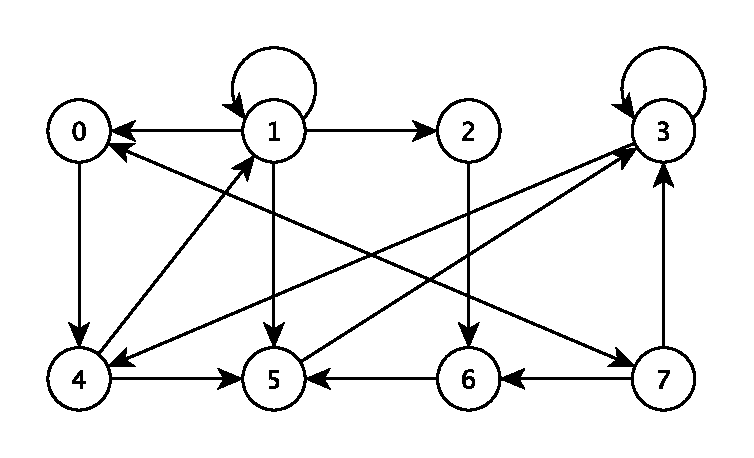
\includegraphics[width=0.99\textwidth]{realNetwork.eps}
        \caption{An example network representation. The circles correspond to the neurons and the arrows between them to directed connection between them.}
		\label{fig-realNetwork}
	\end{subfigure} 
	\quad
	\begin{subfigure}[b]{0.48\linewidth}
		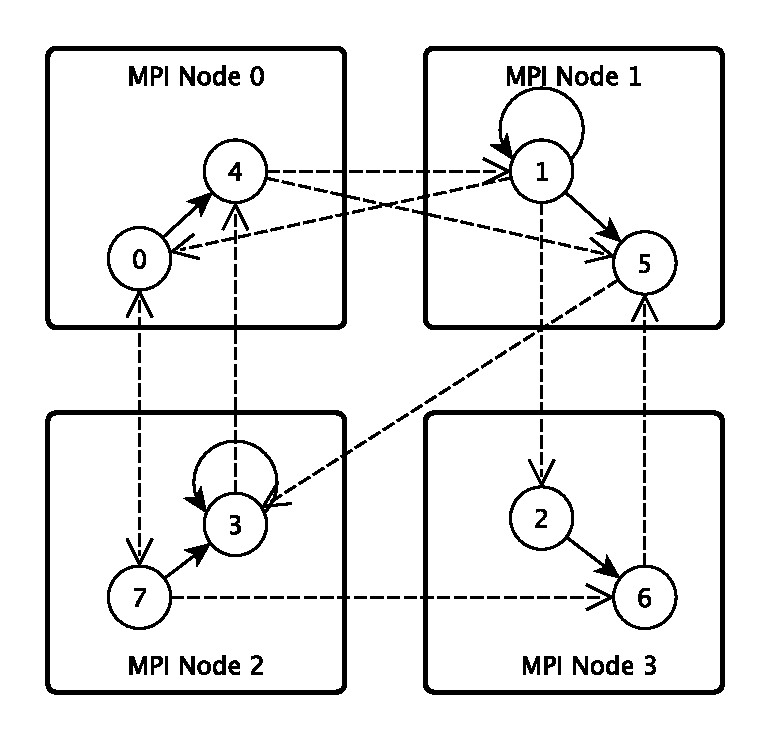
\includegraphics[width=0.99\textwidth]{internalNetwork.eps}
        \subcaption{The internal representation of the network. The circles correspond to the neurons. The rounded boxes represent the individual MPI Nodes. For the distribution the default circular distribution was used. The dashed arrows correspond to asynchronous MPI messages. The normal arrows correspond to internal messages.}
		\label{fig-internalNetwork}
	\end{subfigure}
    \caption{The real and internal representation of a small network.}
\end{figure}


\end{document}

